\section{Operating Charts}
The operating charts describe the modes of operation and the flow of the system without too much detail. Figure~\ref{fig:systemFlowchart} is the system's main flowchart, in it one can see how the devices goes in and out of each of it's operating modes. When the system is powered up it will perform it's Boot Sequence, this includes initializing the MCU and all it's peripherals. Once the Boot Sequence has been completed the device itself will enter Shutdown Mode. In Shutdown Mode the system is operating with very low power listening for a specific RF wake-up signal to further then interact with the user. When the devices receives the correct wake-up signal it will enter Stand-By Mode. On Stand-By the device will establish a ZigBee connection with the base station, once connected the user can then select the next operating mode. The system is not intended for a full power down, but it can occur if the battery is fully drained, in this case when the device is powered back it will initialize it's boot sequence. This is an overall explanation of the system's flow, further explanation can be found in each of the operating modes section.
\begin{figure}[H]
	\centering
	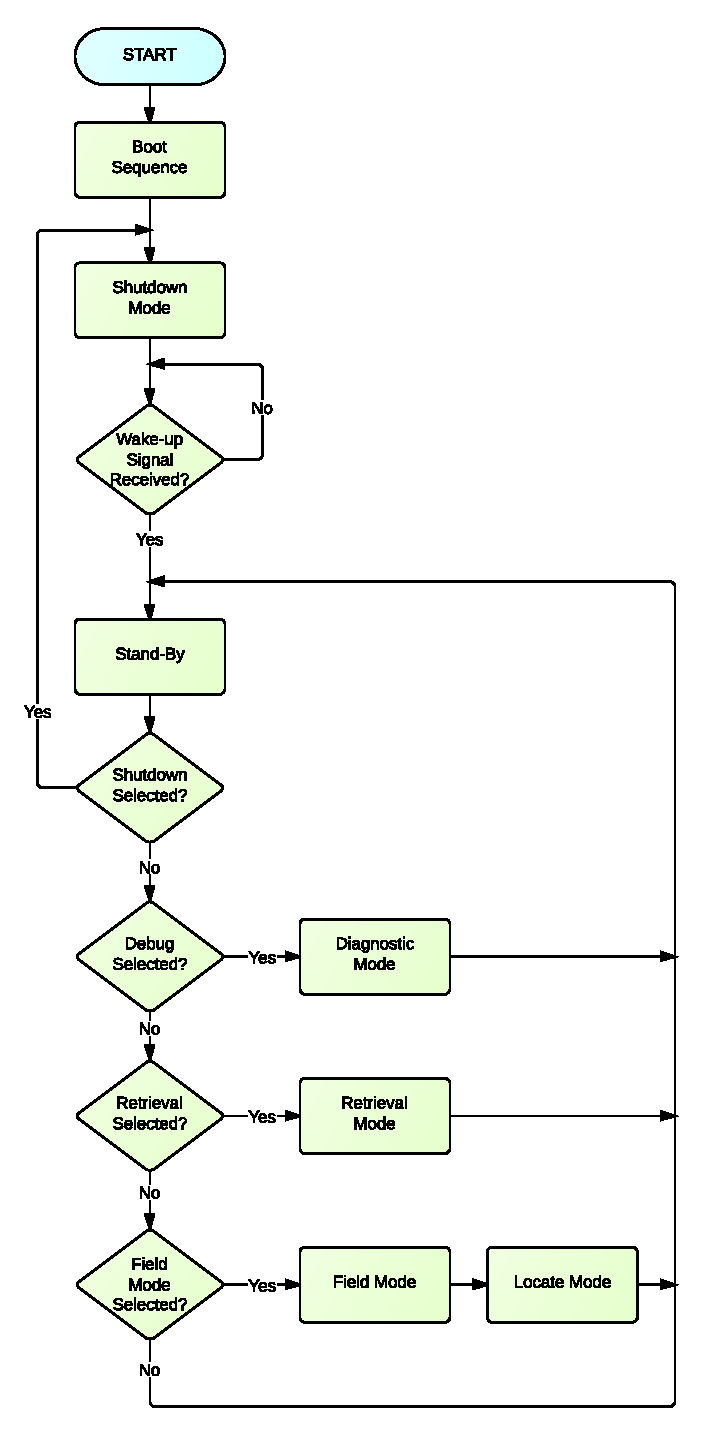
\includegraphics[scale=0.9]{img/SystemFlowchart}
	\caption{System Flowchart \label{fig:systemFlowchart}}
\end{figure}

\subsection{Boot Sequence}
The boot sequence occurs when the device is powered on from a cold power down. The boot sequence contains the functions and routines to initialize the device and it's peripherals. The system power ups and hand shakes with all of it's components for quick test. A successful boot sequence sends the device into Shutdown Mode. However, if any of the components fail to acknowledge and the device is not suited for further a LED indicator will be activated to notify the user.
\begin{figure}[H]
	\centering
	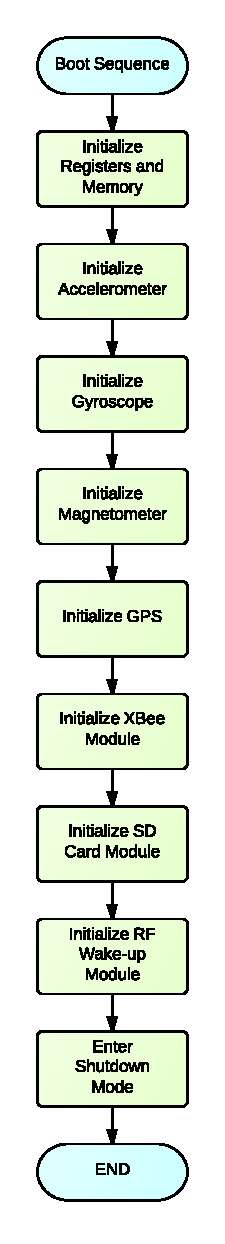
\includegraphics[scale=1.0]{img/BootSequenceFlowchart}
	\caption{Boot Sequence \label{fig:bootSequence}}
\end{figure}

\subsection{Shutdown Mode}
On shutdown mode the device is in deep sleep, the MCU is in low power mode and all components expect one are turned off. The single component that will be on will be the RF Wake-up receiver. The low power ASK receiver will be operating in listening mode. On this mode the receiver is capable of detecting the wake-up carrier, when detected then the receiver sends a interrupt to the MCU waking it up and proceeding to enter Stand-By Mode.
\begin{figure}[H]
	\centering
	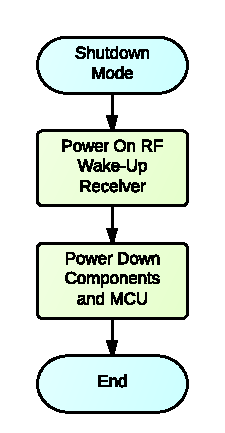
\includegraphics[scale=1.0]{img/ShutdownMode}
	\caption{Shutdown Mode \label{fig:shutdownMode}}
\end{figure}

\subsection{Stand-By Mode}
On Stand-By mode the system is conserving power with some components turned off while maintaining an connection through ZigBee to the base station. On this mode the system is basically waiting for user interaction, the device is connected to the base station and simple information is transmitted to the base station's user interface. The data is Battery and SD Card information. The system is also waiting for the user to select the next operating mode, the use can either test the device with Diagnostic Mode, retrieve it's data with Retrieval Mode or enter Field Mode and run an experiment. The components that are awake on this mode are the SD Card Module and the XBee module.
\begin{figure}[H]
	\centering
	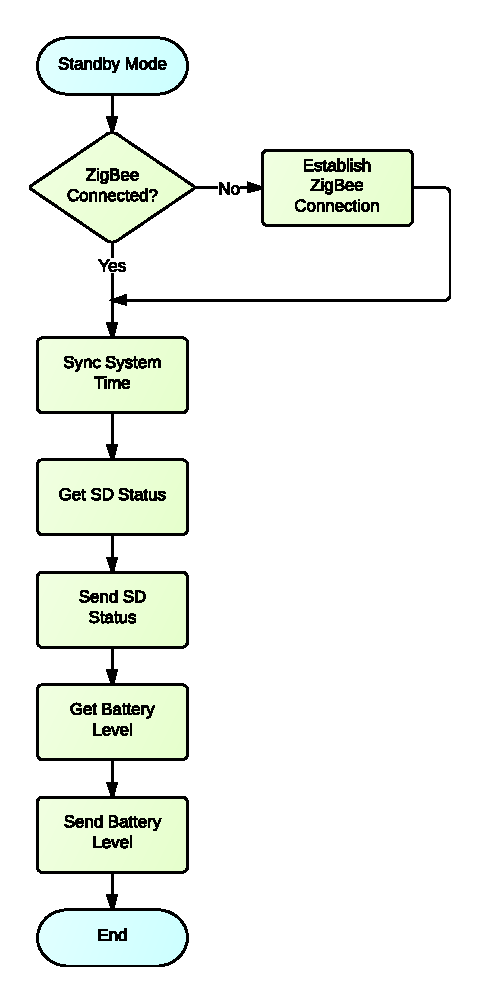
\includegraphics[scale=1.0]{img/StandByMode}
	\caption{Stand-By Mode \label{fig:standByMode}}
\end{figure}

\subsection{Diagnostic Mode}
On Diagnostic Mode the device maintains communication to the base stations and sends real-time information of the different components to the base station, the user can then observe and verify such data.
\begin{figure}[H]
	\centering
	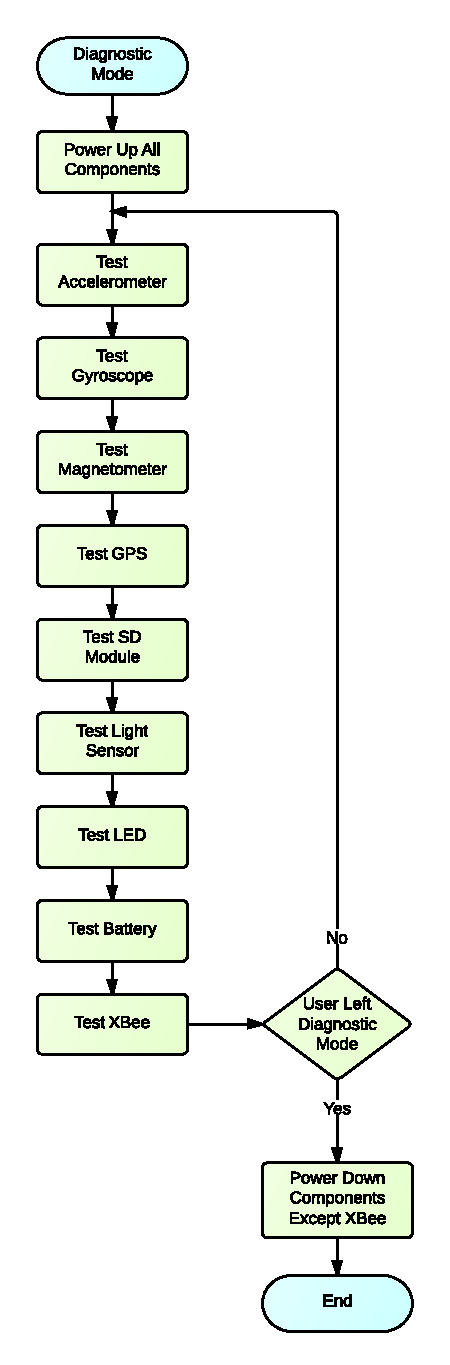
\includegraphics[scale=1.0]{img/DiagnosticMode}
	\caption{Diagnostic Mode \label{fig:diagnosticMode}}
\end{figure}

\subsection{Field Mode}
On Field Mode the device captures data from the accelerometer, gyroscope and magnetometer. The time the system is capturing data is defined by the user trough the base station. On this mode all other components are turned off except those from which data will be captured and the SD Card which is where the data will be saved. Data is captured for the duration of the selected time and data points are saved in the SD card each with a time stamp from which they were captured. Once the data capturing time is over the device automatically start operating in Locate Mode.
\begin{figure}[H]
	\centering
	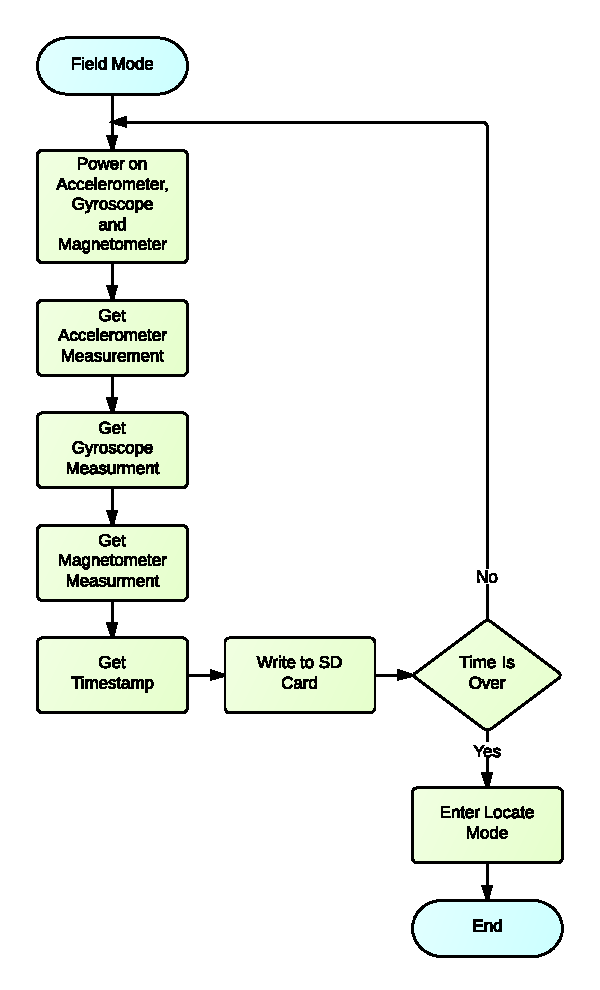
\includegraphics[scale=1.0]{img/FieldMode}
	\caption{Field Mode \label{fig:fieldMode}}
\end{figure}

\subsection{Locate Mode}
On Locate Mode the device is trying to be found by the user. The system turns on the XBee Module and the GPS and turns off all other components. The system then proceeds to try an establish a ZigBee connection to the base station and get a GPS lock. Once the device gets it's location using the GPS Module it will then broadcast such location to the base station trough the ZigBee connection. When the user successfully retrieves the device it can be switched to Stand-By Mode for later use.
\begin{figure}[H]
	\centering
	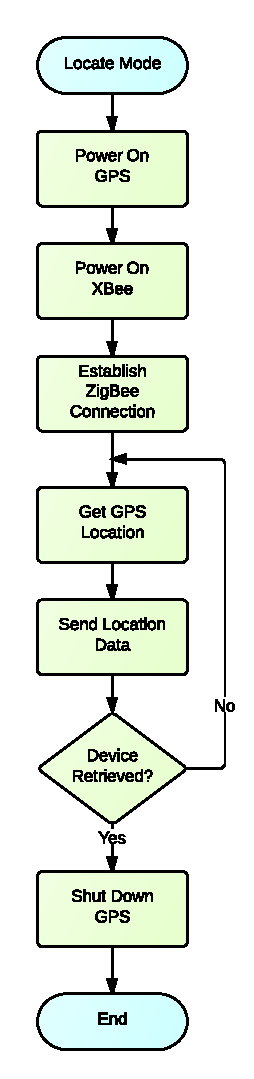
\includegraphics[scale=1.0]{img/LocateMode}
	\caption{Locate Mode \label{fig:locateMode}}
\end{figure}

\subsection{Retrieval Mode}
Retrieval Mode is the operation mode of the device in which the system transfers the collected data from the SD Card to the base station. Data is transfered trough the established ZigBee connection and if desired can be erased from the SD Card.
\begin{figure}[H]
	\centering
	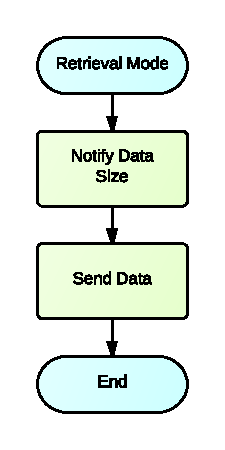
\includegraphics[scale=1.0]{img/RetrievalMode}
	\caption{Retrieval Mode \label{fig:retrivalMode}}
\end{figure}



